\textbf{1. MEDIOS DE TRANSMISIÓN }

El medio de transmisión es el camino físico entre el transmisor y el
receptor. Cualquier medio físico que pueda transportar información en
forma de señales electromagnéticas se puede utilizar en las redes de
datos como un medio de transmisión.

El medio físico puede condicionar la máxima distancia que puede existir
entre los equipos que se intercomunican, velocidad de transferencia
(expresada en número de bits por segundo bps o baudios), topología y el
método de acceso.

Los principales medios de transmisión pueden ser:

• Guiados, cuando las ondas se transmiten confinándolas a lo largo de un
camino (medio) físico como por ejemplo un cable.

• No guiados (inalámbricos), la propagación de la señal se hace a través
del aire, el mar o el espacio.

\textbf{1.1 ALAMBRE DE COBRE}

El cable de par trenzado consiste en grupos de hilos
de~\href{https://es.wikipedia.org/wiki/Cobre}{cobre}~entrelazados en
pares en
forma~\href{https://es.wikipedia.org/wiki/H\%C3\%A9lice_(geometr\%C3\%ADa)}{helicoidal}.
Esto se hace porque dos alambres paralelos constituyen una antena
simple. Cuando se entrelazan los alambres helicoidalmente, las ondas se
cancelan, por lo que la interferencia producida por los mismos es
reducida lo que permite una mejor transmisión de datos.

Así, la forma entrelazada permite reducir la interferencia eléctrica
tanto exterior como de pares cercanos y permite transmitir datos de
forma más fiable. Un cable de par trenzado está formado por un grupo de
pares entrelazados (normalmente 2, 4 o 25 pares), recubiertos por un
material~\href{https://es.wikipedia.org/wiki/Aislamiento_el\%C3\%A9ctrico}{aislante}.
Cada uno de estos pares se identifica mediante un color.

Cable de par trenzado:~Forma de conexión en la que dos aisladores son
entrelazados para tener menores interferencias y aumentar la potencia y
disminuir la diafonía de los cables adyacentes.

La tasa de trenzado, usualmente definida en vueltas por metro, forma
parte de las especificaciones de un tipo concreto de cable. Cuanto menor
es el número de vueltas, menor es la atenuación de la diafonía. Donde
los pares no están trenzados, como en la mayoría de las conexiones
telefónicas residenciales, un miembro del par puede estar más cercano a
la fuente que el otro y, por tanto, expuesto a niveles ligeramente
distintos de IEM.

Está limitado en distancia, ancho de banda y tasa de datos. También hay
que destacar que la atenuación es una función fuertemente dependiente de
la frecuencia. La interferencia y el ruido externo también son factores
importantes, por eso se utilizan coberturas externas y el trenzado. Para
señales analógicas se requieren amplificadores cada 5 o 6 kilómetros,
para señales digitales cada 2 o 3. En transmisiones de señales
analógicas punto a punto, el ancho de banda puede llegar hasta 250 kHz.
En transmisión de señales digitales a larga distancia, la velocidad de
datos no es demasiado grande, no es muy efectivo para estas aplicaciones
o dispositivos En redes locales que soportan ordenadores locales, la
velocidad de datos puede llegar a 10 Mbps (Ethernet) y 100 Mbps (Fast
Ethernet).

En el cable par trenzado de cuatro pares, normalmente solo se utilizan
dos pares de conductores, uno para recibir (cables 3 y 4) y otro para
transmitir (cables 1 y 2), aunque no se pueden hacer las dos cosas a la
vez, teniendo una trasmisión half-dúplex. Si se utilizan los cuatro
pares de conductores la transmisión es full-dúplex.

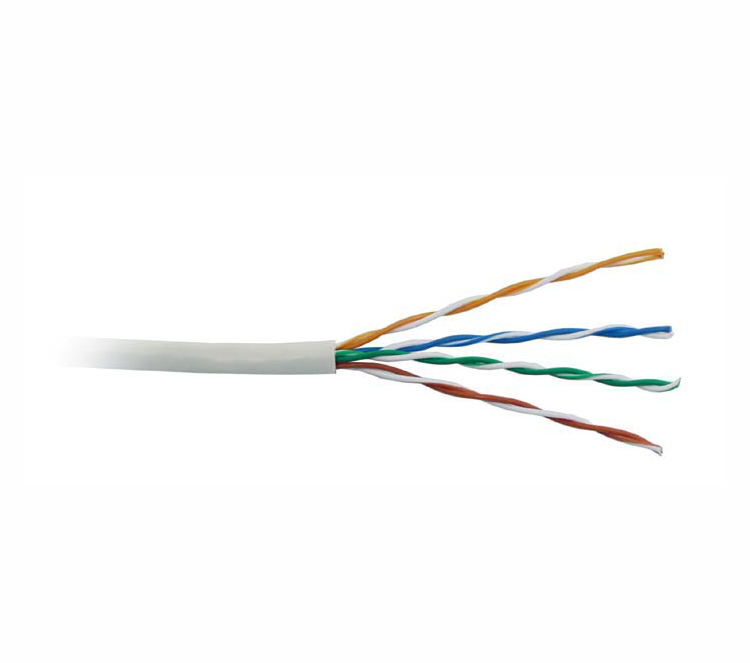
\includegraphics[width=5.09375in,height=2.54167in]{./media/media/image1.jpeg}

\textbf{1.2 CABLE COAXIAL}

El cable coaxial es otro medio de comunicación de datos ampliamente
usado. Está compuesto por un cable de cobre (conductor interno), rodeado
por un material aislante (llamado ``shell''), que a su vez está envuelto
por un segundo conductor (usualmente una maya de alambres finos) que le
da al cable mayor~protección electromagnética que la del cable de par
trenzados. Finalmente, el cable está cubierto por un material plástico
llamado ``jacket''. El cable coaxial, también llamado coax, es un medio
de alta amplitud de banda que puede llevar miles de señales a la vez.
Este tipo de cable puede transmitir datos a mayor distancia que el cable
de par trenzado y es menos susceptible a la interferencia que el STP. El
cable coaxial permite dos tipos de transmisiones: transmisión de base
ancha (broadband) y transmisión de banda-base (baseband).

\begin{quote}
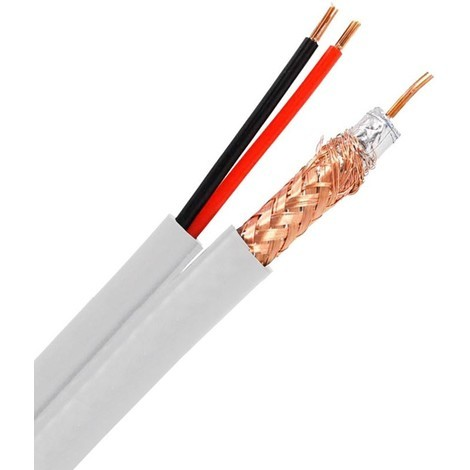
\includegraphics[width=4.25000in,height=3.42708in]{./media/media/image2.jpeg}
\end{quote}

En la transmisión de base ancha (broadband) un solo cable es dividido
eléctricamente en muchos canales, cada uno llevando diferentes
transmisiones. Esta transmisión es análoga. Utiliza una onda de
transmisión de alta frecuencia, la que se divide en amplitudes de bandas
separadas por los protectores de banda (guardbands) para prevenir
interferencia entre las señales. Usando transmisión de base ancha, una
compañía de televisión por cable puede transmitir múltiples canales a
los hogares individuales mediante un solo cable. Similarmente, el cable
de banda ancha puede transmitir voz, video, datos y otras señales.

~

El otro tipo de transmisión es la banda-base (baseband). En ésta, solo
una señal se transmite a través del cable. Las computadoras utilizan la
transmisión de banda-base para enviar datos a otras computadoras en una
red local. La transmisión de banda-base es digital. El cable y los
conectores usados son menos costosos que los de transmisión de base
ancha.

~

La alta amplitud de banda del cable coaxial lo hace muy atractivo para
una gran variedad de usos. En el pasado, el cable coaxial era usado
principalmente para transmisiones de radio y televisión por cable y para
enlaces entre computadoras y sus equipos auxiliares. Según ha aumentado
la necesidad de líneas de teléfonos adicionales, se ha ido utilizando el
cable coaxial para comunicación~telefónica y de datos.

Sin embargo, el cable coaxial es menos utilizado que el UTP en redes de
área local (LAN), pues el UTP es menos costoso y más fácil de manejar e
instalar. Otra desventaja del cable coaxial es su tamaño, pues es mucho
más grande y pesado que el cable de par trenzado y cable de fibra
óptica.

\textbf{1.3 GUÍA DE ONDA}

Una guía de onda es cualquier estructura física que guía ondas
electromagnéticas. El medio dieléctrico en el que esta propagación se
produce está limitado, ya sea por un material conductor (microondas y
radiofrecuencia) o por otro dieléctrico (para frecuencias ópticas).

Dado que la energía se transporta por ondas electromagnéticas, las
características de las guías de onda tales como impedancia, potencia y
atenuación se expresan tales como campos eléctricos y magnéticos
característicos.

Algunos sistemas de telecomunicaciones utilizan la propagación de ondas
en el espacio libre, sin embargo, también se puede transmitir
información mediante el confinamiento de las ondas en cables o guías. En
altas frecuencias las líneas de transmisión y los cables coaxiales
presentan atenuaciones muy elevadas por lo que impiden que la
transmisión de la información sea la adecuada, son imprácticos para
aplicaciones en HF(alta frecuencia) o de bajo consumo de potencia,
especialmente en el caso de las señales cuyas longitudes de onda son del
orden de centímetros, esto es, microondas.

La transmisión de señales por guías de onda reduce la disipación de
energía, es por ello que se utilizan en las frecuencias denominadas de
microondas con el mismo propósito que las líneas de transmisión en
frecuencias más bajas, ya que se presentan poca atenuación para el
manejo de señales de alta frecuencia.

Las paredes conductoras del tubo confinan la onda al interior por
reflexión, debido a la ley de Snell en la superficie, donde el tubo
puede estar vacío o relleno con un dieléctrico. El dieléctrico le da
soporte mecánico al tubo (las paredes pueden ser delgadas), pero reduce
la velocidad de propagación.

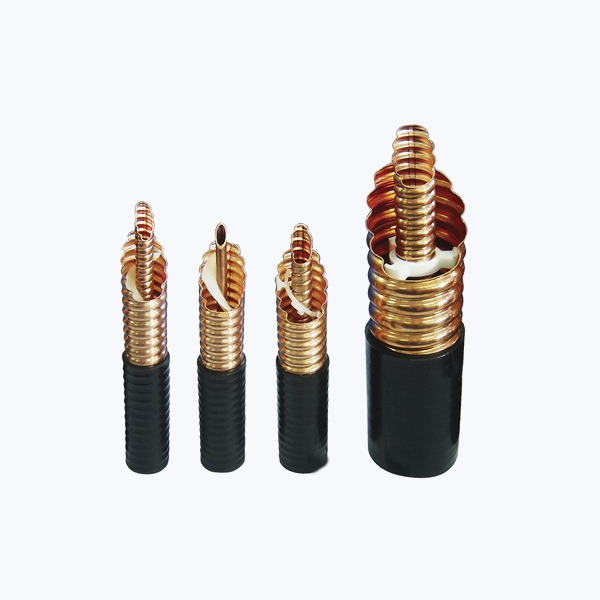
\includegraphics[width=3.89583in,height=3.64583in]{./media/media/image3.jpeg}

En las guías, los campos eléctricos y los campos magnéticos están
confinados en el espacio que se encuentra en su interior, de este modo
no hay pérdidas de potencia por radiación y las pérdidas en el
dieléctrico son muy bajas debido a que suele ser aire. Este sistema
evita que existan interferencias en el campo por otros objetos, al
contrario de lo que ocurría en los sistemas de transmisión abiertos.

La guía de onda se puede visualizar de manera simplificada en la figura
a continuación, suponiendo que está formada por dos láminas conductoras
y que el transporte de la energía se lleva a cabo mediante reflexiones
continuas y no por medio de corrientes superficiales como en el caso de
las líneas de transmisión.

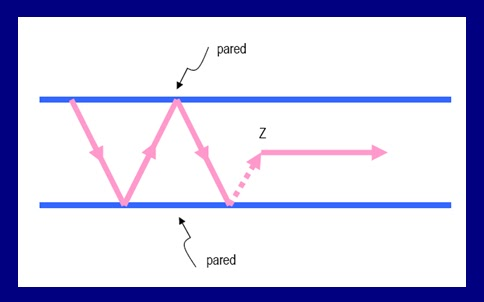
\includegraphics[width=5.04167in,height=3.14583in]{./media/media/image4.jpeg}

\textbf{1.4 FIBRA ÓPTICA}

El cable de fibra utiliza luz para transmitir las señales de datos. La
luz transmite señales digitales usando impulsos de luz para representar
0 y 1. El cable de fibra óptica está compuesto de uno o más cables
pequeños de vidrio o plástico. Cada cable, llamado fibra óptica, es tan
fino como un cabello humano. De hecho, un cable de fibra óptica está
compuesto de muchas fibras ópticas, cada uno rodeada de una barrera de
reflexión~(``cladding''); sobre esta barrera está otra que protege a la
fibra óptica; también se incluye una fibra para fortalecer el cable; y
finalmente una cobertura exterior llamada ``jacket''.

~

La mayor diferencia entre el cable de fibra óptica y el par trenzado o
el cable coaxial es la manera en que las señales de voz y datos se
transmiten. Los cables de cobre transmiten señales eléctricas, mientras
que los cables de fibra óptica transmiten señales por medio de ondas
luminosas (luz). El cable de fibra óptica utiliza un diodo emisor de luz
(LED -- Light-emitting diode) o un láser para enviar pulsos de luz a
través de las fibras. Un LED es una luz de bajo poder creado por un
diodo eléctrico, del mismo tipo de luz usado en algunos relojes
digitales. Un láser provee una fuente de luz más poderosa que el LED,
pero también más costosa. La luz permite que la velocidad de transmisión
de la fibra óptica sea mucho mayor que la del cable de par trenzado o
del cable coaxial.

~

Los cables de fibra óptica están disponibles en tres tipos, que varían
de acuerdo al método usado para transmitir la luz por el cable:

~

\begin{enumerate}
\def\labelenumi{\arabic{enumi}.}
\item
  Fibra multi-modal de índice escalonado (Multimode step index) --
  Utiliza una cobertura plástica o un ``cladding'' parecido a un espejo
  alrededor del cable para reflejar la luz desde el láser o LED. Según
  la luz es reflejada por los lados del cable, se mueve en el cable
  hasta su destino.
\item
  Fibra multi-modal de índice gradual (Multimode graded index) -- En
  este tipo de fibra óptica el núcleo está hecho de varias capas
  concéntricas de material óptico con diferentes índices de refracción.
  El cable varía en densidad, lo que ocasiona curvatura en la luz. Tanto
  el fenómeno de curvatura como el de reflexión causan que la luz se
  mueva hacia el receptor.
\item
  Fibra mono-modal (Single-mode cable) -- Es el tipo de cable más
  rápido. Utiliza un cable muy delgado rodeado por una envoltura que
  concentra el calor. Su principal diferencia es que envía la luz en
  forma directa sin necesidad de reflexión en las paredes de los cables.
\end{enumerate}

Ambos cables de multimodo reflejan la luz a lo largo de la envoltura
mediante el efecto de reflexión (rebote) para transmitir la luz a través
del cable. Es posible que algunos rayos de luz se salgan del patrón de
rebote. Estos rayos viajan mayor distancia y por más tiempo para
alcanzar el final del cable. Esto resulta en pérdida de fortaleza en la
señal (attenuation) y en la dispersión de la señal transmitida.

~

Ventajas del cable de fibra óptica:

\begin{enumerate}
\def\labelenumi{\arabic{enumi}.}
\item
  Alta velocidad de transmisión -- puede transmitir a 100 Mbps, y sigue
  aumentando.
\item
  Seguridad -- Interceptar un cable de cobre es relativamente fácil,
  permitiendo que se pueda robar datos sin que se conozca que está
  ocurriendo. Interceptar un cable de fibra óptica es prácticamente
  imposible, dado su composición. Y si se pudiera, es fácil detectarlo
  por la interrupción de la luz.
\item
  Inmunidad a la interferencia eléctrica
\end{enumerate}

~

Por lo general, la fibra óptica es usada para enlazar redes como LAN,
WAN u otros. Típicamente no se utilizan para enlazar PC individuales a
LAN por el alto costo de las tarjetas de interfase para las PC.
Excepciones a esta regla incluyen ambientes en donde la PC está a más de
100 metros (382 pies) de la conexión de LAN más cercana, ambientes en
donde la interferencia electromagnética es un problema y ambientes en
los cuales es crucial la seguridad.

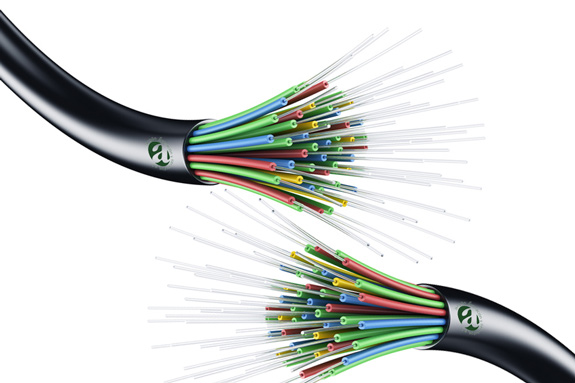
\includegraphics[width=5.90556in,height=3.93333in]{./media/media/image5.jpeg}

\textbf{1.5 LED}

Iluminación led se está convirtiendo en tecnología popular de hoy, y es
utilizada para iluminar hogares, edificios, empresas, negocios, etc. La
tecnología Lifi pretende usar este tipo de iluminación para transmitir
información hacia cualquier dispositivo perceptible a la luz led o que
esté dentro del área de incidencia de esta, mediante cambios de
intensidad de la luz. Por tanto, la tecnología lifi consiste en
transmitir información por medio de la luz led.

Lifi es un tipo de conexión a Internet que usa tecnología que se
caracteriza por transmitir información a través de la luz led que podría
llegar a los 10 Gbps de velocidad. Esto porque la luz se enciende y
apaga hasta 10 mil millones de veces por segundo, lo que hace que se
transforme la información en forma binaria (0 y 1); se aprovecha esta
característica para poder enviar la información a través de la onda de
la luz.

Esta tecnología OWC utiliza la luz de diodos emisores de luz (leds) como
medio de comunicación para redes, móviles, comunicaciones de alta
velocidad, de manera similar a wifi. En el año 2013 se preveía que el
mercado de lifi crecería a una tasa anual compuesta de 82 \% entre 2013
y 2018, para convertirse en un nicho de mercado de más de 6000 millones
de dólares en menos de cuatro años.

Las comunicaciones de luz visible trabajan a modo de parpadeo,
conectando y apagando la corriente a los leds a tal velocidad, que es
imperceptible para el ojo humano. La transmisión de datos a través de
ledes mediante el uso de lifi obligaría a mantener encendidas las
bombillas, pudiéndose atenuar su luminosidad hasta no ser visibles para
el ojo humano y continuaría estando operativa la comunicación. El no
atravesar las ondas de luz las paredes hace que la distancia en las
comunicaciones sean más cortas (pero por sensores se soluciona este
pequeño problema) pero a la misma vez evita muchos problemas de
piratería, al contrario que la comunicación wifi. Tampoco es necesaria
la comunicación en modo línea de visión directa para transmitir la
señal, la luz se refleja en las paredes alcanzando una velocidad de 70
Mbit/s.

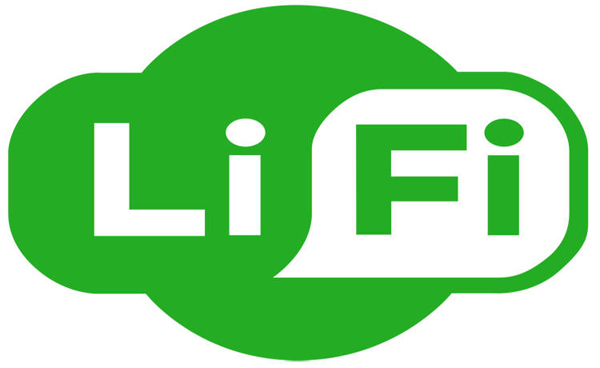
\includegraphics[width=5.90556in,height=3.62222in]{./media/media/image6.jpeg}

Una de las ventajas de la tecnología lifi es la de poder utilizarse en
zonas sensibles a las áreas electromagnéticas, como puede ser cabinas de
aviones, hospitales y centrales nucleares, sin causar interferencias
electromagnéticas. Ambas conexiones (wifi y lifi) utilizan el espectro
electromagnético para la transmisión de datos, pero mientras que wifi
utiliza ondas de radio, lifi utiliza la luz visible. Según la Comisión
Federal de Comunicaciones (Federal Communications Commission, FCC) de
los Estados Unidos, mientras el espectro electromagnético para el wifi
se está saturando, lifi casi no tiene limitaciones de capacidad. Esto es
debido a que el espectro de luz visible es 10 000 veces más largo que
todo el espectro de radiofrecuencias completo. Las sucesivas
investigaciones indican que se están alcanzando velocidades de
transmisión superior a 10 Gbit/s, mucho más rápida que las primeras
mediciones realizadas desde banda ancha durante el año 2013. Una de sus
principales características es que va a resultar diez veces más barato
que la tecnología wifi.

Algunas de las ventajas que podemos citar son:

\begin{itemize}
\item
  La velocidad de transmisión de datos es muy alta puede ir desde los 15
  Mb/s hasta los 20 Gb/s.
\item
  No existe la interferencia con elementos de radio frecuencia ya que su
  medio de trasmisión es la luz, por lo que se puede usar en lugares
  donde el wifi no llega
\item
  No requiere de circuitos ni antenas o receptores complejos, ya que
  lifi utiliza métodos de modulación parecidos a los infrarrojos
\item
  Al mismo tiempo que se ilumina un lugar se puede tener señal de lifi,
  lo que supondría un ahorro de energía
\item
  Puede permitir conexiones bajo el agua o en aviones, y otros lugares
  donde ahora no se puede tener señal.
\end{itemize}

Aún existen algunas desventajas dentro de las que podemos destacar:

\begin{itemize}
\item
  Las ondas de luz visible no traspasan objetos, como sí lo hacen las
  ondas de radio, por lo que si existe una interferencia se pierde la
  señal
\item
  El alcance del haz de luz de los leds no es muy amplio, pues sólo
  alcanza 5 ó 10 metros.
\end{itemize}

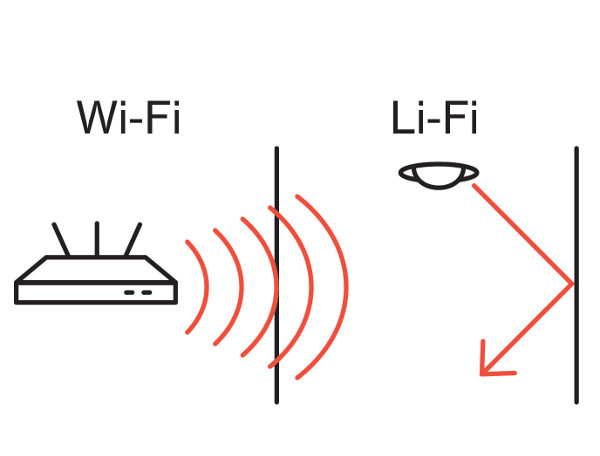
\includegraphics[width=5.90556in,height=4.48819in]{./media/media/image7.jpeg}

\textbf{1.6 LASER}

La transmisión de enormes masas de datos está haciendo llegar a sus
límites la capacidad de la radiofrecuencia, por lo que empresas de todo
el mundo están trabajando en una tecnología láser que pueda servir como
sustituta, una idea que suena a una película de ciencia ficción más que
a la realidad.

La principal ventaja de las emisiones láser es precisamente su mayor
capacidad. Mientras que el récord mundial de la radiofrecuencia es de 36
gigabits por segundo (4,5 GB por segundo), los investigadores del Centro
Aeroespacial de Alemania (DLR, por sus siglas en alemán), ubicado cerca
de Múnich, consiguieron con láser un volumen de 1,7 terabits por segundo
(212,5 GB por segundo).

``En el caso de la radiofrecuencia hay un límite físico, pero la
frecuencia es mucho más elevada en el caso del láser'', explica Wolfram
Peschko, presidente del consejo de administración de Mynaric AG, una
firma surgida del DLR y que está investigando esta técnica para
transformarla en la forma de compartir datos del futuro.

``Partimos de una base muy distinta que las clásicas empresas espaciales
que viven de grandes encargos estatales y fabrican productos
individuales muy costosos'', comenta Peschko, agregando que ``cuando
abordan un proyecto dura años y es realmente caro. Venimos del área
financiada a nivel privado, nuestros tiempos de desarrollo son
relativamente cortos''.

Entre los interesados figuran grandes compañías de alcance mundial como
Facebook, Google y SpaceX, la compañía espacial de Elon Musk, y es que
la cantidad de datos transmitidos a nivel global aumenta constantemente.
``La necesidad actual es de unos 10 gigabits por segundo (1,25 GB por
segundo), pero en un par de años será probablemente de 100 gigabits
(12,5 GB)'', estima Peschko.

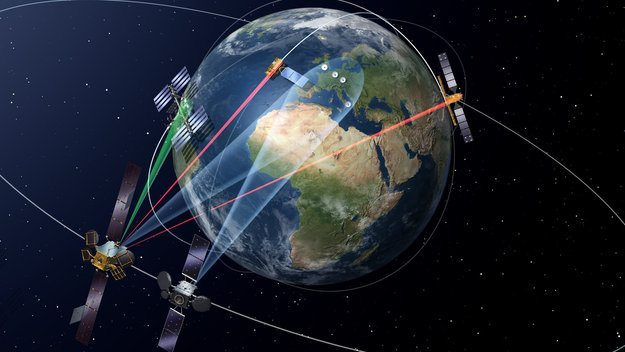
\includegraphics[width=5.90556in,height=3.32569in]{./media/media/image8.jpeg}

Otro factor es el costo, ya que la comunicación inalámbrica láser es
además mucho más barata que la fibra óptica. ``Si hay que pasar todo
bajo tierra, el proceso es muy caro. Las redes en el aire con ayuda de
nuestra tecnología son hasta 10 veces más baratas que las redes clásicas
que van por el suelo''.

La transmisión óptica es posible en múltiples variantes: desde el
satélite o un avión al suelo o desde un satélite a otro o de un avión a
otro. ``Necesitamos un internet alternativo en el aire'', afirma Markus
Knapek, también del consejo de administración de Mynaric.

\textbf{1.7 MICROONDAS}

Además de su aplicación
en~\href{https://es.wikipedia.org/wiki/Horno_microondas}{hornos
microondas}, las microondas permiten transmisiones tanto con antenas
terrestres como con satélites. Dada sus frecuencias, del orden de 1 a
10~Ghz, las microondas son muy direccionales y solo se pueden emplear en
situaciones en que existe una línea visual entre emisor y receptor. Los
enlaces de microondas permiten grandes velocidades de transmisión, del
orden de 10 Mbps.

Comunicación vía microondas.~Básicamente un enlace vía microondas
consiste en tres componentes fundamentales: el transmisor, el receptor y
el canal aéreo. El transmisor es el responsable de modular una señal
digital a la frecuencia utilizada para transmitir, el canal aéreo
representa un camino abierto entre el transmisor y el receptor, y como
es de esperarse el receptor es el encargado de capturar la señal
transmitida y llevarla de nuevo a señal digital.

El factor limitante de la propagación de la señal en enlaces microondas
es la distancia que se debe cubrir entre el transmisor y el receptor,
además esta distancia debe ser libre de obstáculos. Otro aspecto que se
debe señalar es que en estos enlaces, el camino entre el receptor y el
transmisor debe tener una altura mínima sobre los obstáculos en la vía,
para compensar este efecto se utilizan torres para ajustar dichas
alturas.

\subsubsection{Algunas de las ventajas}\label{algunas-de-las-ventajas}

\begin{itemize}
\item
  \begin{quote}
  Antenas relativamente pequeñas son efectivas.
  \end{quote}
\item
  \begin{quote}
  A estas frecuencias las ondas de radio se comportan como ondas de luz,
  por ello la señal puede ser enfocada utilizando antenas parabólicas y
  antenas de embudo, además pueden ser reflejadas con reflectores
  pasivos.
  \end{quote}
\item
  \begin{quote}
  Otra ventaja es el ancho de banda, que va de 2 a 24 GHz.
  \end{quote}
\end{itemize}

\subsubsection{Desventajas}\label{desventajas}

Las frecuencias son susceptibles a un fenómeno llamado~Disminución de
Multicamino~(Multipath Fanding), lo que causa profundas disminuciones en
el poder de las señales recibidas.

A estas frecuencias las pérdidas ambientales se transforman en un factor
importante, la absorción de potencia causada por la lluvia puede afectar
dramáticamente el comportamiento del canal.

\textbf{1.8 SATÉLITES }

Comunicación por Satélites. Un satélite es transportado a su órbita
abordo de un~\href{https://www.ecured.cu/Cohete}{cohete}~capaz de
alcanzar la~\href{https://www.ecured.cu/Velocidad}{velocidad}~suficiente
requerida para no verse influenciado por
el~\href{https://www.ecured.cu/index.php?title=Campo_gravitatorio_terrestre\&action=edit\&redlink=1}{campo
gravitatorio terrestre}.

Una vez conseguido esto, es virtualmente posible conseguir cualquier
plano o altitud de la órbita mediante la utilización de modernos
cohetes. El plano de la órbita se denomina inclinación.

Velocidad de la órbita:

Un satélite puede permanecer en su órbita sólo si su velocidad es lo
suficientemente mayor como para vencer
la~\href{https://www.ecured.cu/Gravedad}{gravedad}~y menor que la
requerida para escapar de la gravedad. La velocidad del satélite es pues
como un compromiso entre esos dos factores, pero ha de ser absolutamente
precisa para la altitud elegida.

V=K/(sqrt(r+a)) Km/s

donde:

V=a velocidad de la órbita en kilómetros por segundo.

a=altitud de la órbita sobre la superficie de la tierra, en Km.

r=el radio medio de la tierra, aproximadamente 6371Km.

K=630

Aunque la tierra no es perfecta y su radio puede variar, vamos a tomar
que posee un valor de 6371Km.

Periodo de la órbita:

El periodo que posee un satélite viene dado por la siguiente fórmula:

P=K(r+a/r)3/2 minutos~donde P=periodo de una órbita en minutos.
a=altitud de la órbita sobre la superficie terrestre. r=radio medio de
la tierra. K=84.49.

Comunicación por Satélites

En las comunicaciones por satélite, las ondas electromagnéticas se
transmiten gracias a la presencia en el espacio de satélites
artificiales situados en órbita alrededor de la Tierra.

Un satélite actúa básicamente como un repetidor situado en el espacio:
recibe las señales enviadas desde la estación terrestre y las reemite a
otro satélite o de vuelta a los receptores terrestres. En realidad, hay
dos tipos de satélites de comunicaciones:

\begin{itemize}
\item
  Satélites pasivos. Se limitan a reflejar la señal recibida sin llevar
  a cabo ninguna otra tare.
\item
  Satélites activos. Amplifican las señales que reciben antes de
  reemitirlas hacia la Tierra. Son los más habituales y son puestos en
  órbita mediante cohetes espaciales que los sitúan circundando la
  Tierra a distancias relativamente cercanas fuera de la atmósfera.
\end{itemize}

A principios de 1960,
la~\href{https://www.ecured.cu/index.php?title=American_Telephone\&action=edit\&redlink=1}{American
Telephone}~and~Telegraph Company (AT\&T)~publicó estudios, indicando que
unos cuantos satélites poderosos, de diseño avanzado, podían soportar
más tráfico que toda la red AT\&T de larga distancia. El costo de estos
satélites fue estimado en solo una fracción del costo de las facilidades
de~\href{https://www.ecured.cu/index.php?title=Microondas_terrestres\&action=edit\&redlink=1}{microondas
terrestres}~equivalentes.

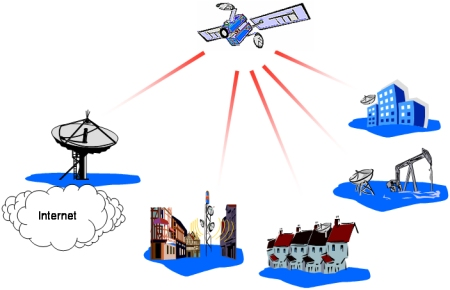
\includegraphics[width=4.68750in,height=3.02083in]{./media/media/image9.jpeg}

A través de los años, los precios de la mayoría de los bienes y
servicios han aumentado sustancialmente; sin embargo, los servicios de
comunicación, por satélite, se han vuelto mas accesibles cada año. En la
mayoría de los casos, los sistemas de satélites ofrecen mas flexibilidad
que los cables submarinos, cables subterráneos escondidos, radio de
microondas en línea de vista, radio de dispersión troposférica, o
sistemas de~\href{https://www.ecured.cu/Fibra_\%C3\%B3ptica}{fibra
óptica}.

Esencialmente, un satélite es
un~\href{https://www.ecured.cu/index.php?title=Repetidor_de_radio\&action=edit\&redlink=1}{repetidor
de radio}~en el cielo (transponder). Un sistema de satélite consiste de
un transponder, una estación basada en tierra, para controlar el
funcionamiento y una red de usuario, de las estaciones terrestres, que
proporciona las facilidades para transmisión y recepción de tráfico de
comunicaciones, a través del sistema de satélite. Las transmisiones de
satélites se catalogan como bus o carga útil. La de bus incluye
mecanismos de control que apoyan la operación de carga útil. La de carga
útil es la información del usuario que será transportada a través del
sistema. Aunque en los últimos años los nuevos servicios de datos
y~\href{https://www.ecured.cu/index.php?title=Radioemisi\%C3\%B3n_de_televisi\%C3\%B3n\&action=edit\&redlink=1}{radioemisión
de televisión}~son mas y más demandados, la transmisión de las señales
de teléfono de voz convencional (en forma analógica o digital).

\textbf{2. ATENUACIÓN}

La energía de una señal decae con la distancia. La~atenuación~es la
perdida de la potencia de una señal. por ello para que la señal llegue
con la suficiente~energía~es necesario el uso de amplificadores
o~repetidores~~ La~atenuación~se incrementa con la frecuencia, con la
temperatura y con el tiempo.

AFECTA:

La atenuación es la razón principal de que el largo de las redes tenga
varias restricciones. Si la señal se hace muy débil, el equipo receptor
no interceptará bien o no reconocerá esta información. Esto causa
errores, bajo desempeño al tener que transmitir la señal.

\textbf{2.1 BOBINA DE CARGA}

La bobina de Pupin o bobina de carga es un inductor que colocado a
intervalos regulares a lo largo de un circuito telefónico formado por
hilos de cobre hace que disminuya la atenuación y la distorsión de
retardo del circuito en la gama de las frecuencias vocales, con el
consiguiente aumento del alcance de la comunicación.

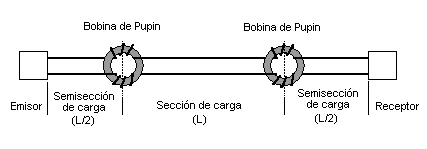
\includegraphics[width=4.44792in,height=1.55208in]{./media/media/image10.png}

Este, en sus estudios sobre los problemas de transmisión del cable
submarino telegráfico trasatlántico, llegó a determinar la condición que
debía cumplir un medio de transmisión ideal. Esta condición, que se
denominó Condición de Heaviside, en esencia afirma que:

\emph{R.C = L.G}

donde R, C, L y G son las constantes primarias del circuito y
representan respectivamente:

R = Resistencia kilométrica en ohmios.

C = Capacidad kilométrica en faradios.

L = Inductancia kilométrica en henrios.

G = Conductancia kilométrica entre hilos del circuito en siemens.

Cuando se cumple la condición de Heaviside la atenuación es mínima e
independiente de la frecuencia, no hay distorsión lineal y el tiempo de
propagación es constante.

En los antiguos circuitos telefónicos de hilo de cobre desnudo de 2 o 3
mm de diámetro, tendidos sobre aisladores, esta condición se cumplía con
cierta aproximación para las frecuencias vocales. El problema surgió con
los cables de pares trenzados, donde R es muy alta al ser los
conductores de menor diámetro, C también es alta al estar muy próximos
entre sí debido al trenzado, en tanto que L es pequeña y G muy pequeña
(el aislamiento entre conductores es muy alto).

Para tratar de cumplir la condición de Heaviside el único parámetro
sobre el que se podía actuar era L.

Para aumentarlo, se apuntaron dos procedimientos:

\begin{itemize}
\item
  El denominado Krarupización ideado por el danés Krarup que consistía
  en rodear los conductores de cobre con otro alambre de material
  magnético con lo que aumenta la inductancia del circuito de forma
  homogénea. Este método era extremadamente caro y solo se usó en
  algunos cables submarinos.
\item
  El otro método es la pupinización consistente en aumentar la
  inductancia, de forma distribuida, mediante la inserción a intervalos
  regulares de bobinas Pupin o de carga.
\end{itemize}

\textbf{2.2 REPETIDORES y AMPLIFICADORES}

El repetidor recibe, amplifica y retransmite las señales, con o sin
conversión de frecuencia, procedentes de una estación base (enlace
descendente) y señales procedentes de los equipos móviles en la
dirección opuesta (enlace ascendente) Una ventaja de los repetidores es
que con un equipo podemos dar la extensión de cobertura necesaria de
forma más económica que con un equipo de estación base convencional. Los
repetidores sirven para extender la cobertura de una estación base, pero
no pueden sustituirla, por eso deben estar conectadas siempre a una
estación base. Las aplicaciones típicas de los repetidores son para
hacer llegar la cobertura a túneles, valles e interior de edificios.

En telecomunicaciones, el término repetidor tiene los siguientes
significados normalizados:

• Un dispositivo analógico que amplifica una señal de entrada,
independientemente de su naturaleza (analógica o digital).

• Un dispositivo digital que amplifica, conforma, retemporiza o lleva a
cabo una combinación de cualquiera de estas funciones sobre una señal
digital de entrada para su retransmisión.

Su funcionamiento es el siguiente: toman la señal que circula por una
red y la propagan sin efectuar ningún tipo de traducción o
interpretación de dicha señal. Su efecto sobre el retardo de propagación
de la señal es mínimo.

Dos cables unidos por un repetidor se ven como un mismo cable. Por ello,
sobre ambos debe ir el mismo tipo de red de área local, puesto que los
nodos de ambos segmentos pertenecen a la misma red. Sin embargo, los
cables que unen sí pueden ser diferentes, por ejemplo, coaxial y fibra
óptica.

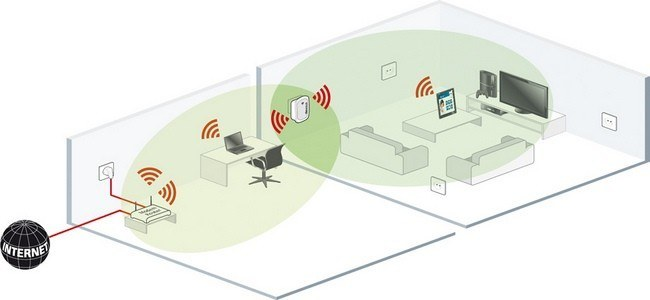
\includegraphics[width=5.90556in,height=2.72569in]{./media/media/image11.jpeg}

Los diferentes tipos de repetidores que nos podemos encontrar en el
mercado, básicamente se pueden clasificar en los siguientes grandes
grupos:

• Repetidores sobre soporte físico

• Repetidores sobre enlace inalámbrico

Repetidores sobre soporte físico

En este caso la estación base se conecta a través del cable o fibra
correspondiente hasta el repetidor de manera que toda la señal de RF
viaja por el soporte físico, convenientemente adaptada para viajar por
este medio. Las principales ventajas de este tipo de repetidores son la
baja atenuación entre la estación base y el repetidor, el aislamiento
total entre el enlace estación base y repetidor y la comunicación entre
el terminal móvil y el repetidor, además no es necesaria una visión
directa entre la estación base y el repetidor. El principal
inconveniente es el elevado coste de implementación.

Según el medio físico que se utilice en los repetidores sobre soporte
físico pueden ser:

• Repetidor sobre cable coaxial

• Repetidor sobre cables de pares

• Repetidor sobre fibra

Repetidores sobre enlace inalámbrico

A diferencia de los anteriores no requiere un soporte físico entre la
estación base donante y el repetidor. Existen dos grandes tipos de
repetidores inalámbricos: los repetidores por radio y los repetidores
por infrarrojos.

Las principales ventajas en este tipo de repetidores son: la
implementación sencilla y rápida, y un menor coste de implementación Los
inconvenientes que nos encontramos con estos repetidores son: una mayor
atenuación entre la estación base y el repetidor y la necesidad de que
tengan visión directa.

\textbf{2.3 ECO}

Cuando hablamos, el sonido de la voz se transmite de la boca
directamente al aire pero parte de él pasa por el cráneo para llegar a
los oídos. A pesar de que casi no se aprecia, este sonido es fundamental
para escucharse a uno mismo y poder, por tanto, tener un tono de voz
natural. Este sonido es conocido en el mundo de las telecomunicaciones
como tono lateral.

Centrándonos en el eco, las palabras que se vierten a la habitación en
la que se produce la conversación, también rebotan contra las paredes y
de nuevo vuelven a los oídos. Si dicho sonido tarda en volver el
resultado será muy molesto. De hecho, cuanto más retardo haya, más
desagradable es la sensación para el oído humano que es muy sensible a
este fenómeno.\\[2\baselineskip]Existen dos tipos de eco a eliminar. El
eco de línea y el digital. El primero es el conocido como eco de línea,
causado por la diafonía en el cableado o en los convertidores. Un eco
que puede llegar a impedir una comunicación de calidad solamente con el
retorno de menos del 1\% del sonido ya que es un incidente muy molesto.

El segundo tipo de eco es el digital, acústico o espacial. Este puede
darse con frecuencia, con todos los problemas que esto conlleva, ya que
el sonido atraviesa varios convertidores hasta llegar a su destino. Cada
uno de ellos requiere su propio tiempo y esto incrementa el riesgo de
aparición de eco porque al expulsarse más tarde el sonido a la
habitación, se produce una reverberación adicional.

La cancelación de ruido a través de la eliminación de los dos ecos.
Llevándolo a la práctica se consigue mediante un dispositivo que detecta
el eco y crea un sonido de contrafase para anularlo.

\textbf{2.4 OPTIMIZAR CANAL}

Las limitaciones de un canal de transmisión, en cuanto al ancho de
banda, dificultad de transmisión, interferencias, y velocidad surgen
mayormente por las características físicas del canal o transmisor
utilizado.

\subsubsection{Ancho de Banda}

En general, una conexión con ancho de banda alto es aquella que puede
llevar la suficiente información como para sostener la sucesión de
imágenes en una presentación de video.

Tener banda ancha implica usar varios servicios de Internet al mismo
tiempo sin que uno afecte a otro. Podemos chatear, navegar por la Web o
hacer una llamada de VoIP y, al mismo tiempo, descargar un archivo de la
Red sin mayores inconvenientes, ya que la mensajería en general requiere
poco ancho de banda. Hay otros servicios que consumen más ancho de
banda, pero que sin una conexión de este tipo serían impensables.

Todo medio de transmisión disminuye el ancho de banda, razón por la cual
toda señal sufre deformación, para transmitir una señal sin deformación
se requiere un ancho de banda infinito.

\subsubsection{Interferencia}

Se presentan cuando se trabaja con dos señales con bandas de frecuencia
muy próximas.~Son mas relevantes en medio no guiados, sin embargo en los
medios guiados, las emisoras de cables cercanos pueden causar
interferencias por lo que es conveniente apantallar el medio guiado que
se utiliza.

Se puede minimizar esto asegurandose de no permitir que las antenas del
receptor se toquen una con otra al colocar los receptores y asegurarse
que ningún transmisor de radio, incluyendo el transmisor del sistema o
aquellos para otros sistemas inalámbricos, esté aproximadamente entre 10
a 15 pies (3 a 4,5 m) de las antenas receptoras inalámbricas.
